

\chapter{변수간 관계}

지금까지 한번에 한 변수만 살펴봤다.
이번장에서 변수간 관계를 살펴본다.
변수 하나를 알고 있는 것이 다른 변수에 대한 정보를 준다면, 두 변수는 관계가 있다.
예를 들어, 신장과 체중은 관계가 있다; 키가 더 큰 사람이 체중이 더 나가는 경향이 있다.
물론, 완벽한 관계는 아니다: 키 작고 뚱뚱한 사람과 키 크고 마른 사람이 있다.
하지만, 다른 사람의 체중을 추측하려고 한다면, 신장 정보를 모르는 것보다 키 정보를 알고 있는 것이
좀더 정확하게 추정하는데 도움이 된다.

\index{성인 체중 (adult weight)}
\index{성인 신장 (adult height)}


이번 장에서 사용되는 코드는 {\tt scatter.py}에 있다.
코드를 다운로드하고 작업하는 것에 대한 정보는 ~\ref{code}을 참조한다.

\section{산점도 (Scatter plots)}
\index{산점도 (scatter plot)}
\index{그림 (plot)!산점도 (scatter)}

관계(relationship)을 확인하는 가장 간단한 방법이 {\bf 산점도 (scatter plot)}다.
하지만, 좋은 산점도를 만드는 것이 항상 쉬운 것은 아니다.
예제로, BRFSS 응답자에 대한 신장과 체중 플롯을 그릴 것이다. (~\ref{lognormal} 절 참조)
\index{BRFSS}

데이터 파일을 읽어서 신장과 체중 정보를 추출하는 코드가 다음에 있다.

\begin{verbatim}
    df = brfss.ReadBrfss(nrows=None)
    sample = thinkstats2.SampleRows(df, 5000)
    heights, weights = sample.htm3, sample.wtkg2
\end{verbatim}

{\tt SampleRows} 함수는 데이터에서 일부를 임으로 골라낸다. 
\index{SampleRows}

\begin{verbatim}
def SampleRows(df, nrows, replace=False):
    indices = np.random.choice(df.index, nrows, replace=replace)
    sample = df.loc[indices]
    return sample
\end{verbatim}

{\tt df}는 데이터프레임이고, {\tt nrows}는 선택할 행의 갯수가 되고, 
{\tt replace}는 복원 추출을 해야 하는지 나타내는 부울(boolean) 표식이다; 
다른 말로, 동일한 행이 한번 이상 선택되어 추출되는지 나타낸다. 

\index{데이터프레임 (DataFrame)}
\index{thinkplot}
\index{부울 (boolean)}
\index{복원 (replacement)}

{\tt thinkplot}에는 {\tt Scatter} 메쏘드가 있는데, 산점도를 그린다.
%
\begin{verbatim}
    thinkplot.Scatter(heights, weights)
    thinkplot.Show(xlabel='Height (cm)',
                   ylabel='Weight (kg)',
                   axis=[140, 210, 20, 200])
\end{verbatim}

그림~\ref{scatter1} (왼쪽)에 관계 형태를 보여주는 결과가 있다.
예상했던 것처럼, 더 키가 큰 사람이 더 체중이 나가는 경향이 있다.

\begin{figure}
% scatter.py
\centerline{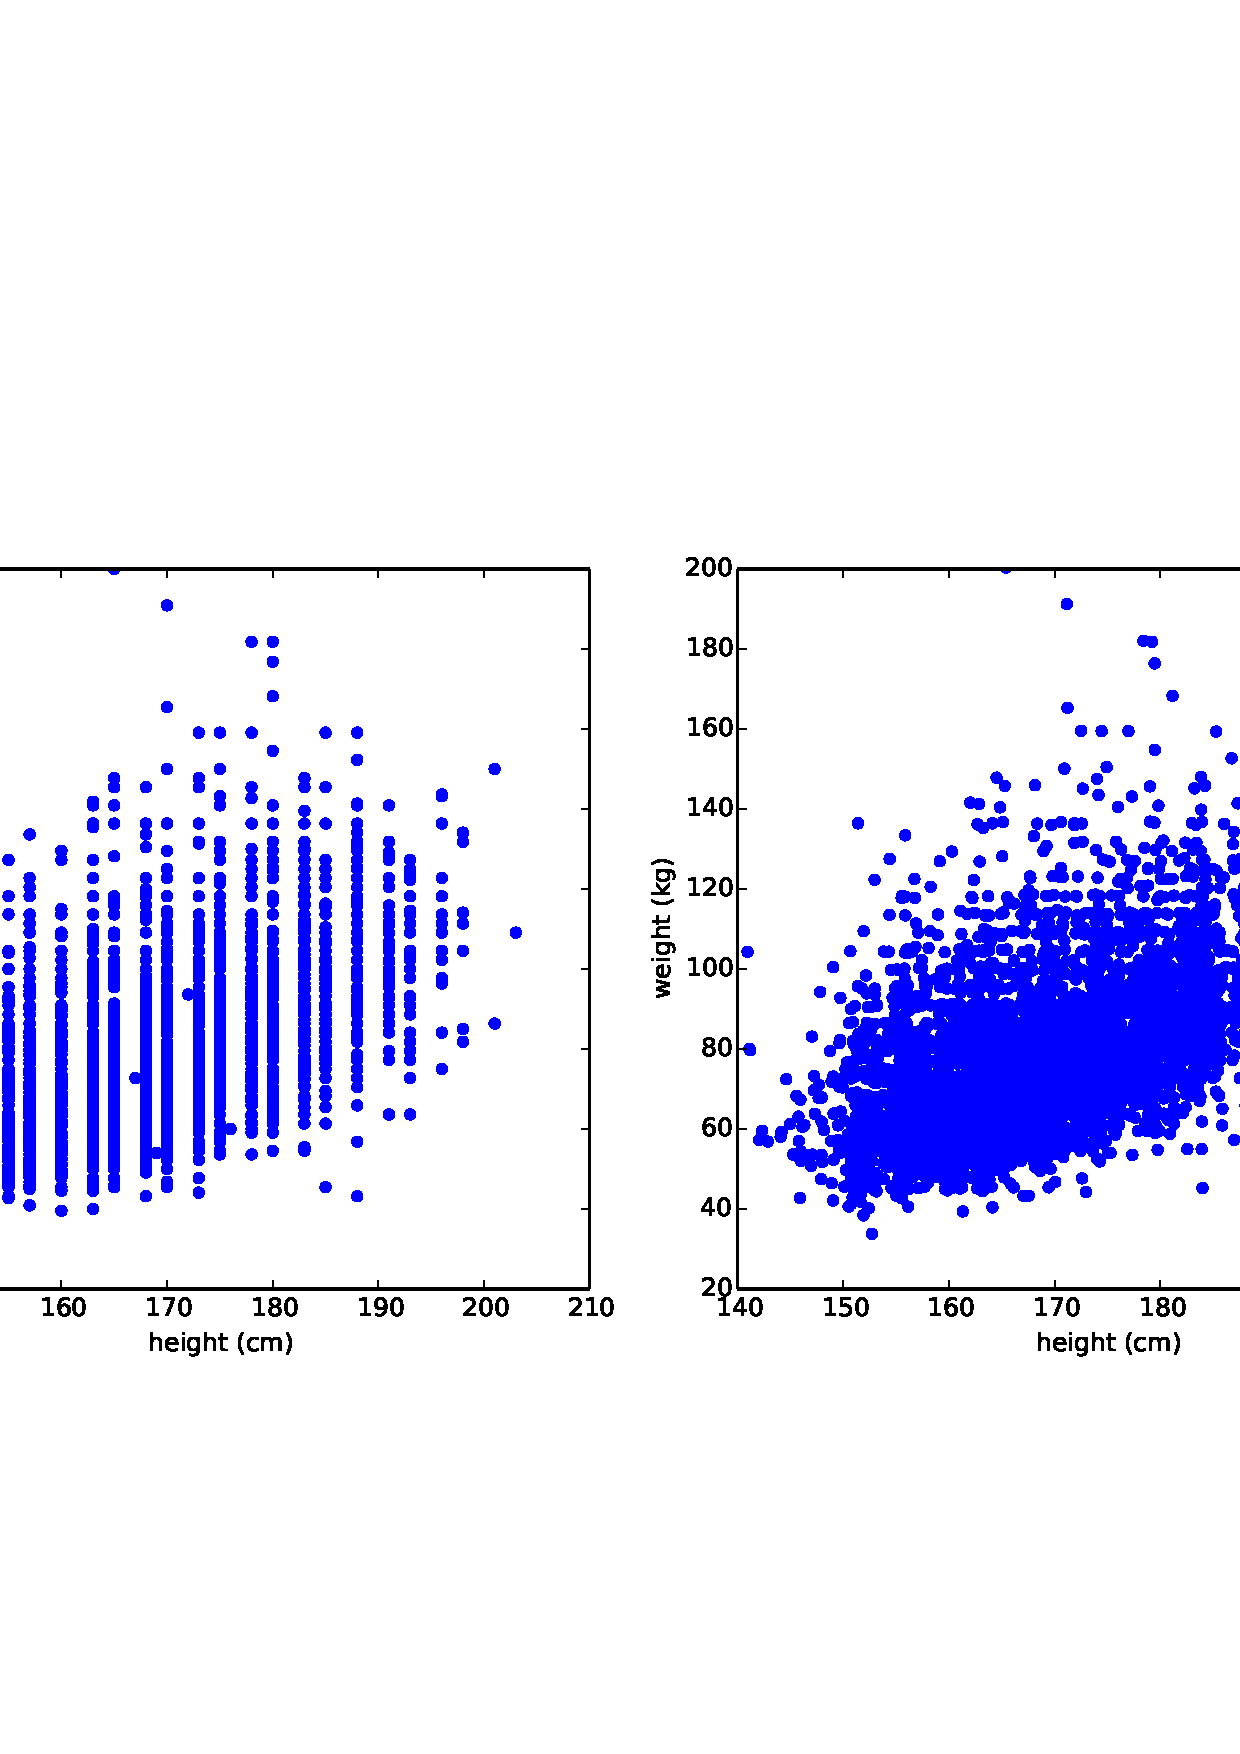
\includegraphics[height=3.0in]{figs/scatter1.pdf}}
\caption{지터되지 않은(좌측), 지터된(우측) 산점도로 BRFSS에서 응답자 신장과 체중을 도식화.}
\label{scatter1}
\end{figure}

하지만, 상기 그림이 데이터를 가장 잘 표현하는 것은 아니다.
이유는 데이터가 열에 떼지어 몰려있다. 문제는 
신장이 가장 가까운 인치(inch) 단위로 반올림되고, 센티미터로 변환하고 나서,
다시 반올림했다. 변환 과정에서 정보가 유실되었다.

\index{신장 (height)} 
\index{체중 (weight)} 
\index{지터 (jitter)}

유실된 정보를 다시 되돌릴 수는 없지만, 데이터를 {\bf 지터링(jittering)}\footnote{jittering, 지터로 번역을 했는데 통계 사전에는 등록이 되어있지 않고 일반 사전에는 ``조금씩 움직이다''라고 나와있다.}해서 
산점도에 효과를 최소화할 수 있다. 반올림 효과를 되돌리도록 확률 잡음(random noise)를 추가한다는 의미다.
측정값이 가장 근사한 인치(inch) 정보로 반올림되어 있어서, 0.5 인치 즉, 1.3 센티미터까지 차이가 생길 수도 있다. 마찬가지로, 체중은 0.5 kg까지 차이가 생길 수 있다. 

\index{균등 분포 (uniform distribution)}
\index{분포 (distribution)!균등 (uniform)}
\index{잡음 (noise)}

%
\begin{verbatim}
    heights = thinkstats2.Jitter(heights, 1.3)
    weights = thinkstats2.Jitter(weights, 0.5)
\end{verbatim}

{\tt Jitter} 함수를 구현한 것이 다음에 있다.

\begin{verbatim}
def Jitter(values, jitter=0.5):
    n = len(values)
    return np.random.uniform(-jitter, +jitter, n) + values
\end{verbatim}

값은 임의 시퀀스가 될 수 있다; 결과는 넘파이(NumPy) 배열이다.
\index{넘파이 (NumPy)}

그림~\ref{scatter1} (오른편)에 결과가 있다.
지터링(jittering)을 통해서 반올림으로 인한 시각적 효과를 줄이고,
관계 형태를 좀더 명확히 한다. 하지만, 일반적으로 시각화 목적으로만
데이터를 지터링해야 하고, 분석을 위해서 지터링된 데이터 사용은 피해야 한다.

지터링 조차도 데이터를 표현하는 가장 최선의 방법이 되지는 못한다.
중복되는 점이 많아서 그림에서 조밀한 부분에 있는 데이터를 숨기고,
균형이 맞지 않게 특이점을 강조한다. 이와 같은 효과를 {\bf 포화 (saturation)}라고 부른다.
\index{특이점 (outlier)}
\index{포화 (saturation)}

\begin{figure}
% scatter.py
\centerline{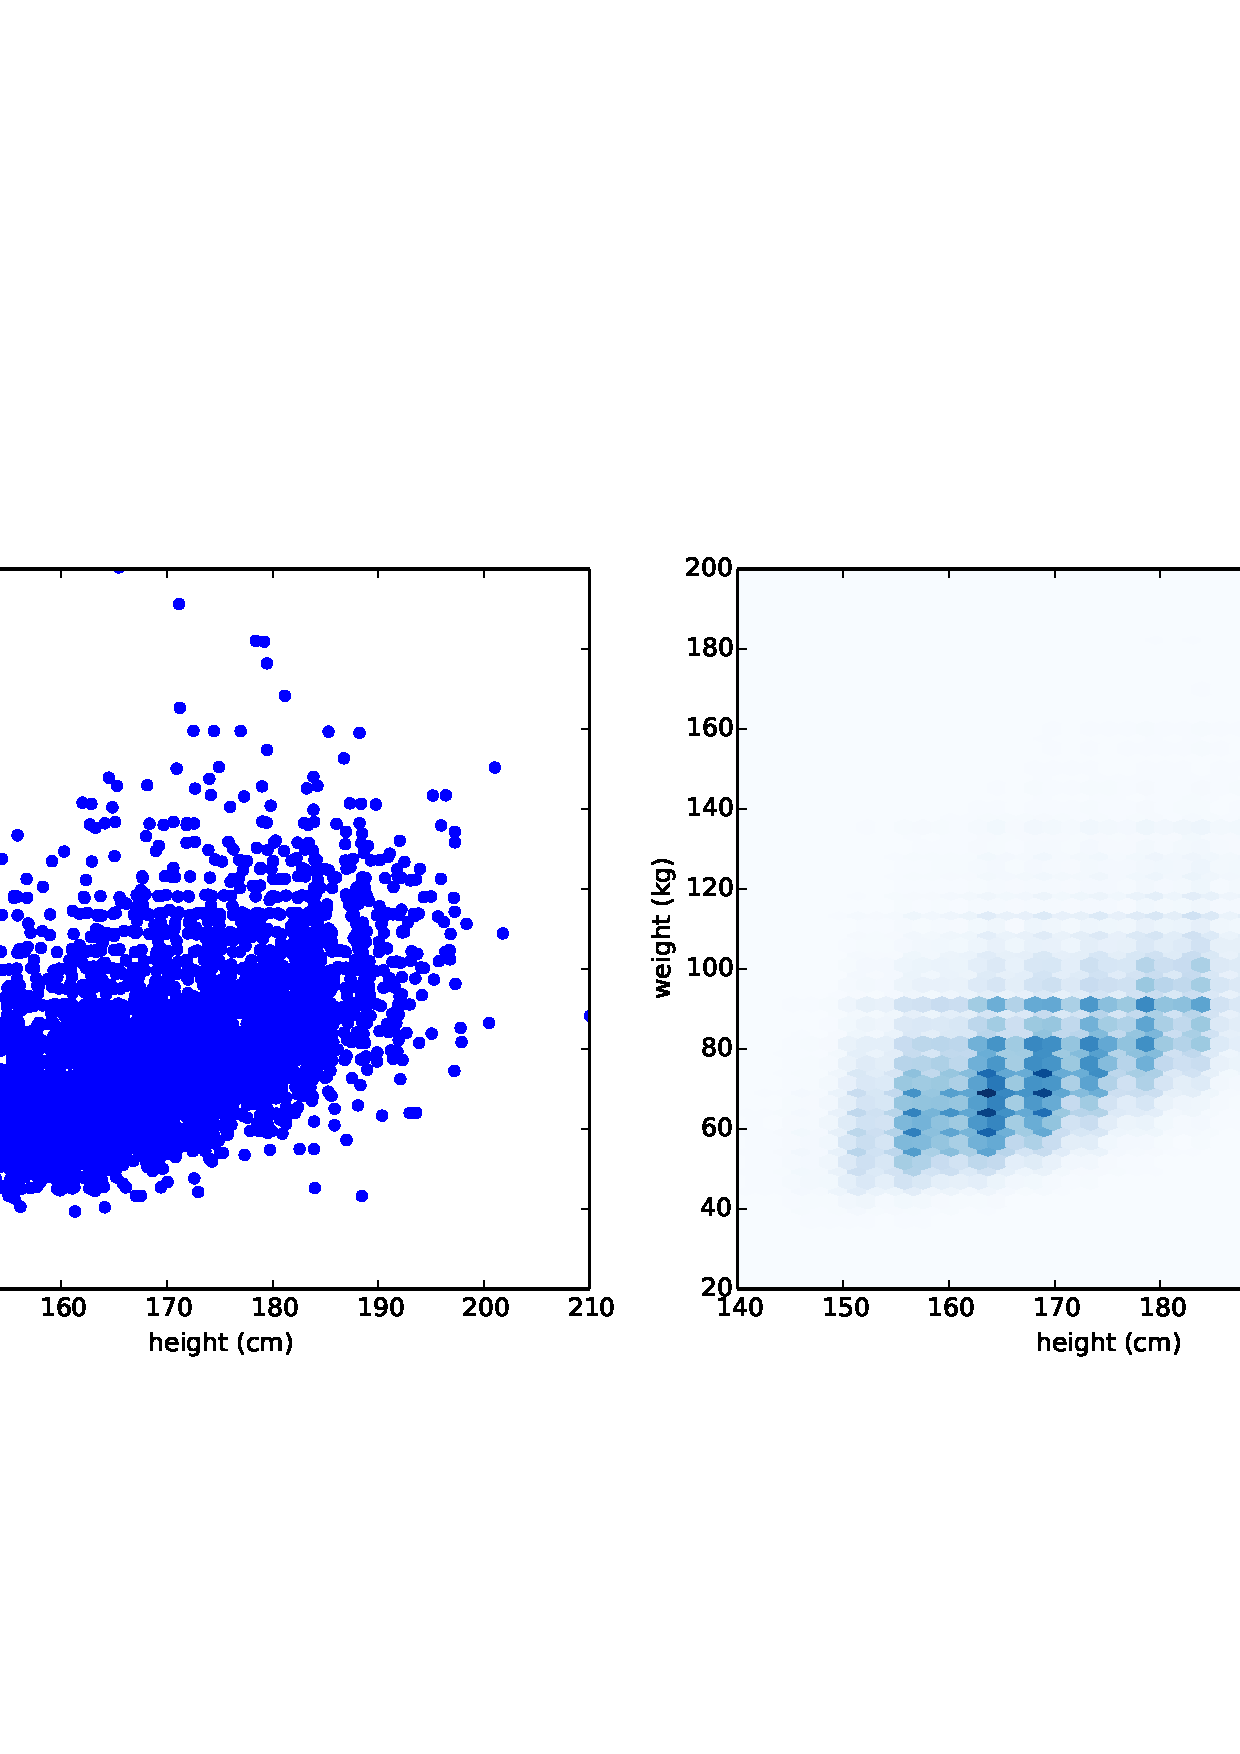
\includegraphics[height=3.0in]{figs/scatter2.pdf}}
\caption{지터되지 않은(좌측), 지터된(우측) 산점도로 BRFSS에서 응답자 신장과 체중을 도식화.}
\label{scatter2}
\end{figure}

이런 문제를 {\tt alpha} 모수로 해결할 수 있는데, 수행하는 역할은 점들을 부분적으로 투명하게 한다.

%
\begin{verbatim}
    thinkplot.Scatter(heights, weights, alpha=0.2)
\end{verbatim}
%

그림~\ref{scatter2} (왼편)에 결과가 있다.
겹쳐지는 데이터 점들이 더 어두워 보여서 색이 짙음이 밀도와 비례하여 균형을 맞춘다. 이 버젼으로 그린 플롯을 살펴보면, 앞에서 명확하지 않은 두가지 자세한 사항을 볼 수 있다; 90 kg 즉, 200 파운드 근처에 수평선과 몇군데 신장에서 수직 군집이 보인다. 데이터가 파운드 단위로 자기 응답에 기반하기 때문에, 가장 그럴듯한 설명은 응답자가 반올림한 값으로 보고를 한 것이다.

\index{thinkplot}
\index{alpha}
\index{투영성 (transparency)}

투명성을 사용해서 중간정도 크기 데이터셋를 처리했다.
하지만, 그림은 단지 BRFSS 자료 414 509 중에서 첫 5000 레코드만 보여준다.

\index{육각함 플롯 (hexbin plot)}
\index{플롯 (plot)!육각함 (hexbin)}

더 커다란 데이터셋을 처리하기 위한,
또 다른 선택지가 육각함 플롯 (hexbin plot)이 된다.
그래프를 육각형 통(hexagonal bin)으로 나누고 각 통을 얼마나 많은 데이터가 들어있는지에 따라 색을 칠한다. {\tt thinkplot}에 {\tt HexBin}메쏘드가 있다.
%
\begin{verbatim}
    thinkplot.HexBin(heights, weights)
\end{verbatim}
%

그림~\ref{scatter2} (오른편)에 결과가 있다.
육각함(hexbin)의 장점은 관계 형태도 보여준다는 것이고,
큰 데이터셋에 대해서도 시간과 파일 크기에 둘 관점에서 효율적이다.
단점은 특이점이 보이지 않는다는 것이다.
 
\index{thinkplot}
\index{특이점 (outlier)}

이 사례를 통해서 강조하고자 하는 것은 오해를 불러 일으키는 산출물 없이 관계를 명확하게 보여주는 산점도를 플롯으로 그리는 것이 쉬운 것은 아니라는 점이다.

\index{산출물 (artifact)}


\section{관계를 특징짓기}
\label{characterizing}

산점도는 변수 사이에 관계에 대한 일반적인 인상을 제공한다. 하지만, 관계 본질에 대한 더 많은 통찰을 주는 
다른 시각화방법이 있다. 한 선택지는 변수를 구간화(binning)하고 다른 변수 백분위수를 플롯으로 그리는 것이다.

\index{구간화 (binning)}

넘파이(NumPy)와 판다스가 데이터를 구간화하는 함수를 제공한다.
\index{넘파이 (NumPy)}
\index{판다스 (pandas)}

\begin{verbatim}
    df = df.dropna(subset=['htm3', 'wtkg2'])
    bins = np.arange(135, 210, 5)
    indices = np.digitize(df.htm3, bins)
    groups = df.groupby(indices)
\end{verbatim}

{\tt dropna} 메쏘드는 호명된 칼럼(열)에서 {\tt nan}가 있는 행을 제거한다. 
{\tt arange} 메쏘드는 135부터 210까지 (210은 포함하지 않고) 5만큼 증가하는 구간을 가진 넘파이 배열을 생성한다.

\index{dropna 메쏘드}
\index{digitize 메쏘드}
\index{NaN}

{\tt digitize} 메쏘드는 {\tt df.htm3}에 있는 각 값을 담고 있는 구간 인텍스를 계산한다.
결과는 정수 인텍스 넘파이(NumPy) 배열이다. 
가장 하위 구간에 속하는 값은 인덱스 0에 매핑된다. 가장 상위 구간에 속하는 값은 {\tt len(bins)}에 매핑된다.

\begin{figure}
% scatter.py
\centerline{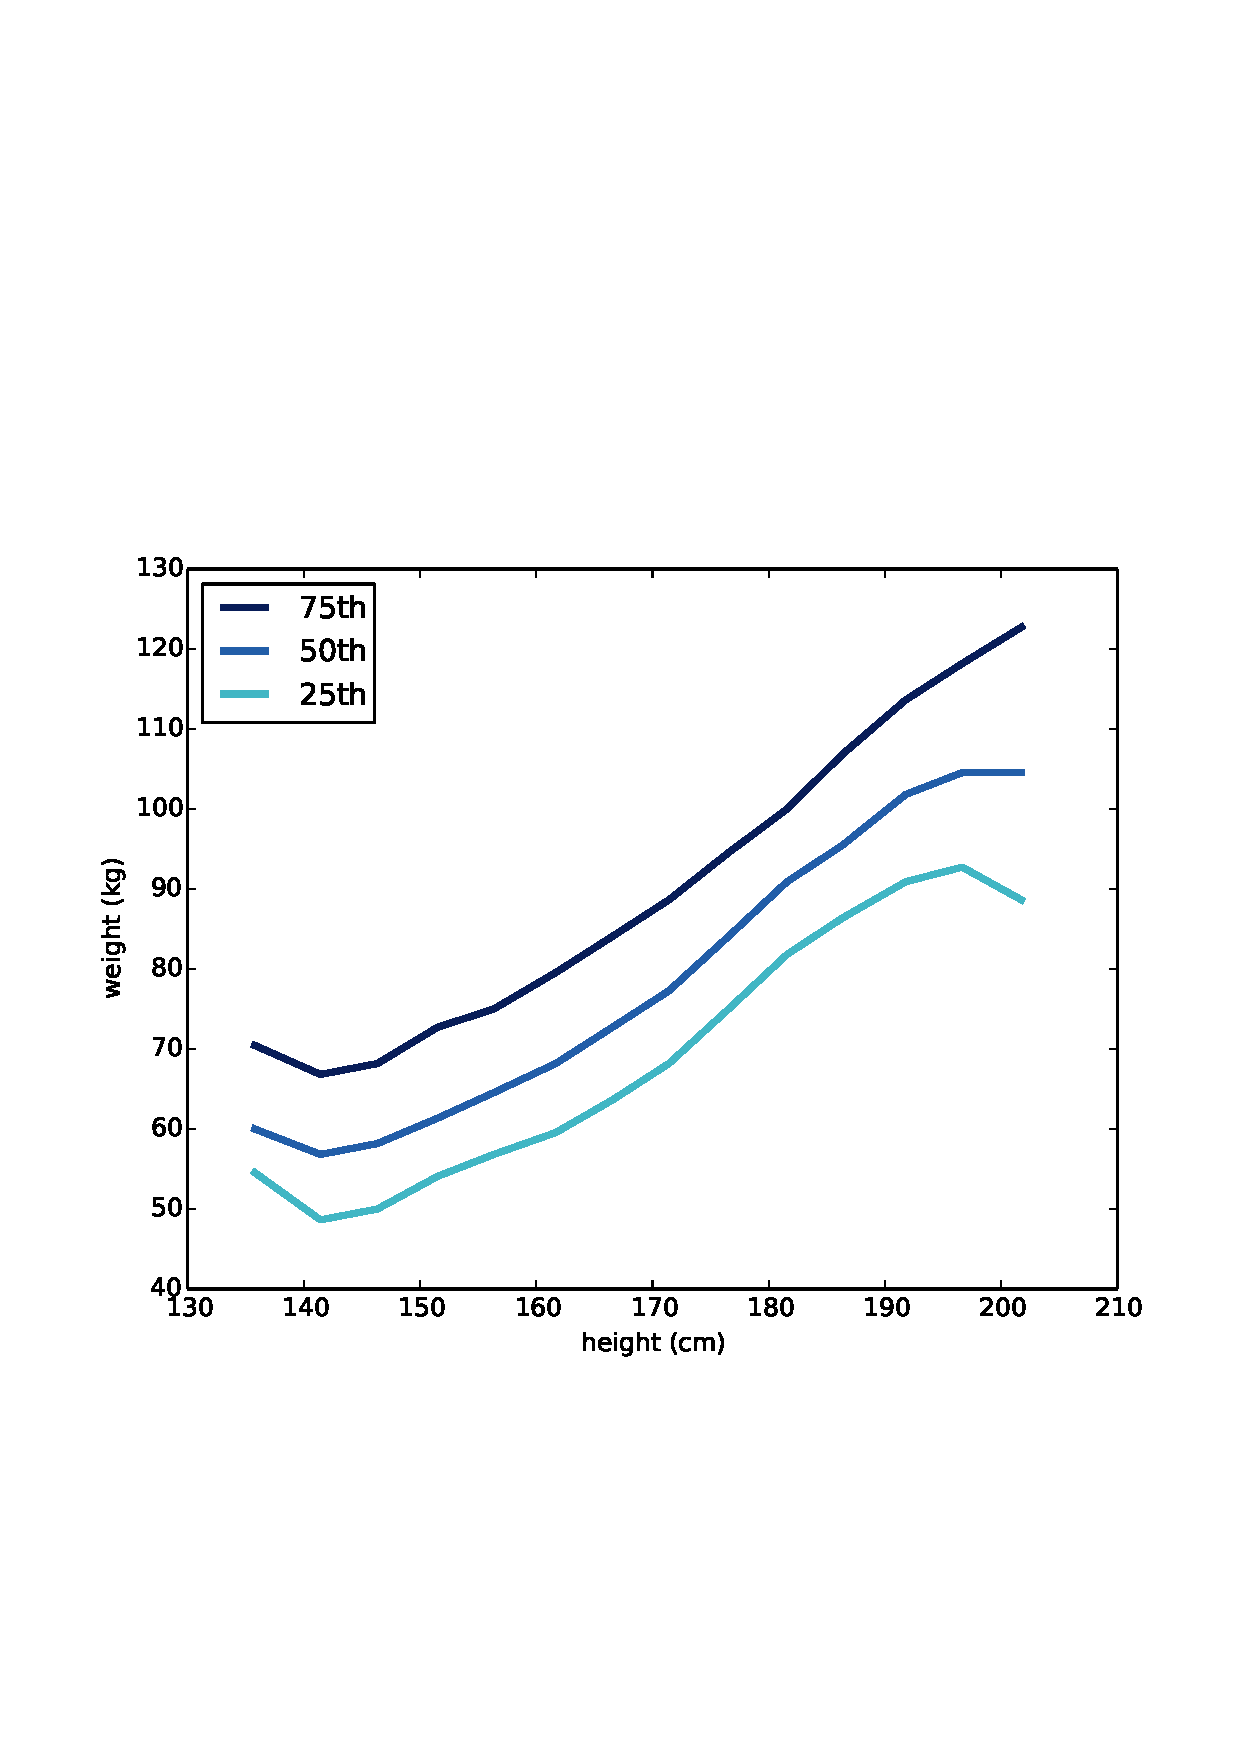
\includegraphics[height=2.5in]{figs/scatter3.pdf}}
\caption{신장 구간 범위에 대한 체중 백분위수.}
\label{scatter3}
\end{figure}

{\tt groupby}는 GroupBy 객체를 반환하는 데이터프레임 메쏘드다;
{\tt for} 루프에 사용되고, {\tt groups}은 그룹 이름과 그룹을 나타내는 데이터프레임을 반복돌린다.
\index{데이터프레임 (DataFrame)}
\index{groupby 메쏘드}

\begin{verbatim}
for i, group in groups:
    print(i, len(group))
\end{verbatim}

이제 각 그룹에 대해서, 평균 신장과 체중 CDF를 계산할 수 있다.
\index{Cdf}

\begin{verbatim}
    heights = [group.htm3.mean() for i, group in groups]
    cdfs = [thinkstats2.Cdf(group.wtkg2) for i, group in groups]
\end{verbatim}

마지막으로, 신장과 체중에 대한 백분위수를 플롯으로 그릴 수 있다.
\index{백분위수 (percentile)}

\begin{verbatim}
    for percent in [75, 50, 25]:
        weights = [cdf.Percentile(percent) for cdf in cdfs]
        label = '%dth' % percent
        thinkplot.Plot(heights, weights, label=label)
\end{verbatim}

그림~\ref{scatter3}에 결과가 나와 있다.
140센티미터에서 200센티미터 사이 두 변수 간의 관계는 대략 선형이다.
이 범위에 99\%이상 데이터가 몰려있다. 그래서, 극단값에 대해서 너무 걱정할 필요는 없다.
\index{thinkplot}


\section{상관 (Correlation)}

{\bf 상관 (correlation)}은 두 변수 간 관계강도를 정량화하는데 사용되는 통계량이다.
\index{상관 (correlation)}

상관을 측정하는데 걸림돌은 비교하려는 변수가 동일한 단위로 표현되지 않는다.
그리고 설사 단위가 동일하다고 하더라도, 다른 분포에서 두 변수가 나왔다.

\index{단위 (units)}

상기 문제에 대한 두가지 일반적인 해결책이 있다.

\begin{enumerate}

\item 각 값을 평균에서 떨어진 표준편차 숫자인 {\bf 표준점수 (standard scores)}로 변환한다. 
이러한 변환은 ``피어슨 곱적률 상관계수 (Pearson product-moment correlation coefficient)''가 된다.
\index{표준점수 (standard score)}
\index{표준편차 (standard deviation)}
\index{피어슨 상관계수 (Pearson coefficient of correlation)}

\item 각 값을 정렬된 리스트 값 인덱스인 {\bf 순위 (rank)}로 변환한다.
이러한 변환은 ``스피어만 순위 상관계수 (Spearman rank correlation coefficient)''가 된다.
\index{순위 (rank)}
\index{백분위수 순위 (percentile rank)}
\index{스피어만 상관계수 (Spearman coefficient of correlation)}

\end{enumerate}

만약 $X$가 일련 $n$개 값, $x_i$라면, 평균을 빼고 표준편차로 나누어서  
표준점수로 전환한다.
$z_i = (x_i - \mu) / \sigma$.
\index{평균 (mean)}
\index{표준편차 (standard deviation)}

분모가 편차다; 평균에서 떨어진 차이. $\sigma$로 나누면 편차를 {\bf 표준화(standardizes)}한다. 그래서 $Z$ 값은 차원이 없다(단위가 없음). 그리고 분포는 평균 0, 분산 1이 된다.
\index{표준화하다 (standardize)}
\index{차이 (deviation)}
\index{정규분포 (normal distribution)}
\index{분포 (distribution)!정규 (normal)}
\index{가우스 분포 (Gaussian distribution)}
\index{분포 (distribution)!가우스 (Gaussian)}

만약 $X$가 정규 분포라면, $Z$도 그렇다. 하지만, 만약 $X$가 기울어지거나 이상점이 있다면, $Z$도 그렇다; 이와 같은 경우, 백분위 순위를 사용하는 것이 좀더 강건하다.
만약 새로운 변수, $R$을 계산한다면, $r_i$는 $x_i$의 순위가 되고, $X$가 무슨 분포든지 관계없이, $R$ 분포는 1에서 $n$까지 균등분포다.

\index{균등분포 (uniform distribution)} 
\index{분포 (distribution)!균등 (uniform)}
\index{강건성 (robust)}
\index{왜도 (skewness)}
\index{이상점 (outlier)}


\section{공분산 (Covariance)}
\index{공분산 (covariance)}
\index{편차 (deviation)}

{\bf 공분산 (Covariance)}은 함께 변화하는 두 변수의 경향성 측도다.
만약 두 변수 계열 $X$ and $Y$가 있다면,
평균에 대한 편자는 다음과 같다.
%
\[ dx_i = x_i - \xbar \]
\[ dy_i = y_i - \ybar \]
%
$\xbar$가 $X$의 표본 평균이고, 
$\ybar$이 $Y$의 표본 평균이다.
만약 $X$와 $Y$가 함께 변한다면, 편차는 동일 기호를 갖는 경향이 있다.

두 변수를 함께 곱한다면, 곱이 양수가 될 때는 편차가 동일한 부호를 갖을 때고, 음수가 될 때는 반대 부호를 갖을 때다.
그래서, 곱을 합하게 되면 함께 변화하는 경향성 측도가 된다. 

공분산은 이들 곱의 평균이다.

%
\[ Cov(X,Y) = \frac{1}{n} \sum dx_i~dy_i \]
%
$n$은 두 계열 변수의 길이다. (두 계열 변수는 길이가 동일해야 한다.)

만약 선형대수학을 공부해따면, {\tt Cov}가 길이로 나눈 편차의 내적(dot product)이다. 그래서 만약 두 벡터가 동일하다면 공분산은 극대화되고, 직교(orthogonal)하면 0, 반대 방향으로 위치하면 부호가 음수가 된다. {\tt thinkstats2}는 {\tt np.dot}을 사용해서 {\tt Cov}를 효과적으로 구현한다.
\index{선형대수학 (linear algebra)}
\index{내적 (dot product)}
\index{직교 벡터 (orthogonal vector)}

\begin{verbatim}
def Cov(xs, ys, meanx=None, meany=None):
    xs = np.asarray(xs)
    ys = np.asarray(ys)

    if meanx is None:
        meanx = np.mean(xs)
    if meany is None:
        meany = np.mean(ys)

    cov = np.dot(xs-meanx, ys-meany) / len(xs)
    return cov
\end{verbatim}

초기 설정값으로 {\tt Cov}가 표본 평균에서 편차를 계산하거나 이미 계산된 평균값을 인자로 넘길 수 있다. 만약, {\tt xs}와 {\tt ys}이 파이썬 시퀀스라면, {\tt np.asarray}가 넘파이(NumPy) 배열로 전환한다.
만약 이미 넘파이(NumPy) 배열이라면, {\tt np.asarray}는 아무 것도 하지 않는다.

\index{넘파이 (NumPy)}

공분산 구현이 설명 목적으로 간단하게 구현되었다.
넘파이(NumPy)와 판다스에 공분산 구현되어 기능을 제공한다.
하지만, 둘다 여기서 다루어지지 않는 작은 표본 크기에 대한 보정기능을 제공한다. 그리고, {\tt np.cov}는 공분산 행렬을 반환하는데, 공분산 행렬은 지금 당장 필요한 것 이상이다.

\index{판다스 (pandas)}


\section{피어슨 상관 (Pearson's correlation)}
\index{상관 (correlation)}
\index{표준 점수 (standard score)}

공분산이 몇몇 연산에서는 유용하지만, 요약 통계량으로는 결코 보고되어지지 않는데 이유는 해석하기기 어렵기 때문이다.
다른 문제점 중에서, 단위가 $X$와 $Y$ 단위의 곱이다.
예를 들어, 이것이 무엇을 의미하든지, BRFSS 데이터셋에서 체중과 신장 공분산은 113 킬로그림-센티미터가 된다.

\index{편차 (deviation)}
\index{단위 (units)}

이 문제에 한 해결책은 표준편차로 편차를 나누고, 표준 점수 곱을 계산하는 것이다.

%
\[ p_i = \frac{(x_i - \xbar)}{S_X} \frac{(y_i - \ybar)}{S_Y} \]
%
$S_X$와 $S_Y$은 $X$와 $Y$의 표준편차다. 이들 곱의 평균은 다음과 같다.

%
\[ \rho = \frac{1}{n} \sum p_i \]
%
혹은 $S_X$ 와 $S_Y$을 빼내서 $\rho$를 다시 작성할 수 있다.
%
\[ \rho = \frac{Cov(X,Y)}{S_X S_Y} \]
%

이 값을 초창기 영향력 있는 통계학자 칼 피어슨(Karl Pearson)을 따라 {\bf 피어슨 상관 (Pearson's correlation)}이라고 부른다.
계산하기 쉽고 해석하기도 쉽다. 표준 점수는 차원이 없어서 $\rho$다.

\index{피어슨, 칼 (Pearson, Karl)}
\index{피어슨 상관계수 (Pearson coefficient of correlation)}

{\tt thinkstats2}에서 구현한 코드가 다음에 있다.

\begin{verbatim}
def Corr(xs, ys):
    xs = np.asarray(xs)
    ys = np.asarray(ys)

    meanx, varx = MeanVar(xs)
    meany, vary = MeanVar(ys)

    corr = Cov(xs, ys, meanx, meany) / math.sqrt(varx * vary)
    return corr
\end{verbatim}

별도로 {\tt np.mean}와 {\tt np.var}을 호출하기 보다 다소 더 효율적으로 {\tt MeanVar}은 평균과 분산을 계산한다.
\index{MeanVar}

피어슨 상관은 항상 -1과 1 사이다. (1,-1을 포함한다.) 만약, $\rho$가 양수라면, 상관이 양(positive)으로 한 변수값이 높으면, 다른 변수값도 높은 경향이 있다는 의미다. $\rho$가 부(negative)이면, 한 변수가값이 높으면, 다른 변수 값은 낮은 경향이 있다는 의미다.

$\rho$ 크기는 상관 강도를 나타낸다. 만약 $\rho$가 1 혹은 -1 이면, 변수는 완벽하게 상관되어 있다는 의미로, 만약 변수 하나를 알고 있다면 다른 하나에 대해서 완벽한 예측이 가능하다는 의미다.
\index{예측 (prediction)}

현실 세계에서 대부분의 상관은 완벽하지 않지만, 여전히 유용하다.
신장과 체중 상관은 0.51로 비슷한 사람과 관련된 변수와 비교하여 볼 때 강한 상관이다.

\section{비선형 관계 (Nonlinear relationships)}

만약 피어슨 상관이 거의 0이라면, 변수 사이에 관계가 없다고 단정하고 싶을 것이다. 하지만, 그러한 결론은 타당하지 않다. 피어슨 상관은 단지 {\em
  선형 (linear)} 관계만을 측정한다. 만약 비선형 관계가 있다면, $\rho$는 비선형 강도를 과소평가하게 된다.

\index{선형 관계 (linear relationship)}
\index{비선형 (nonlinear)}
\index{피어슨 상관 계수 (Pearson coefficient of correlation)}

\begin{figure}
\centerline{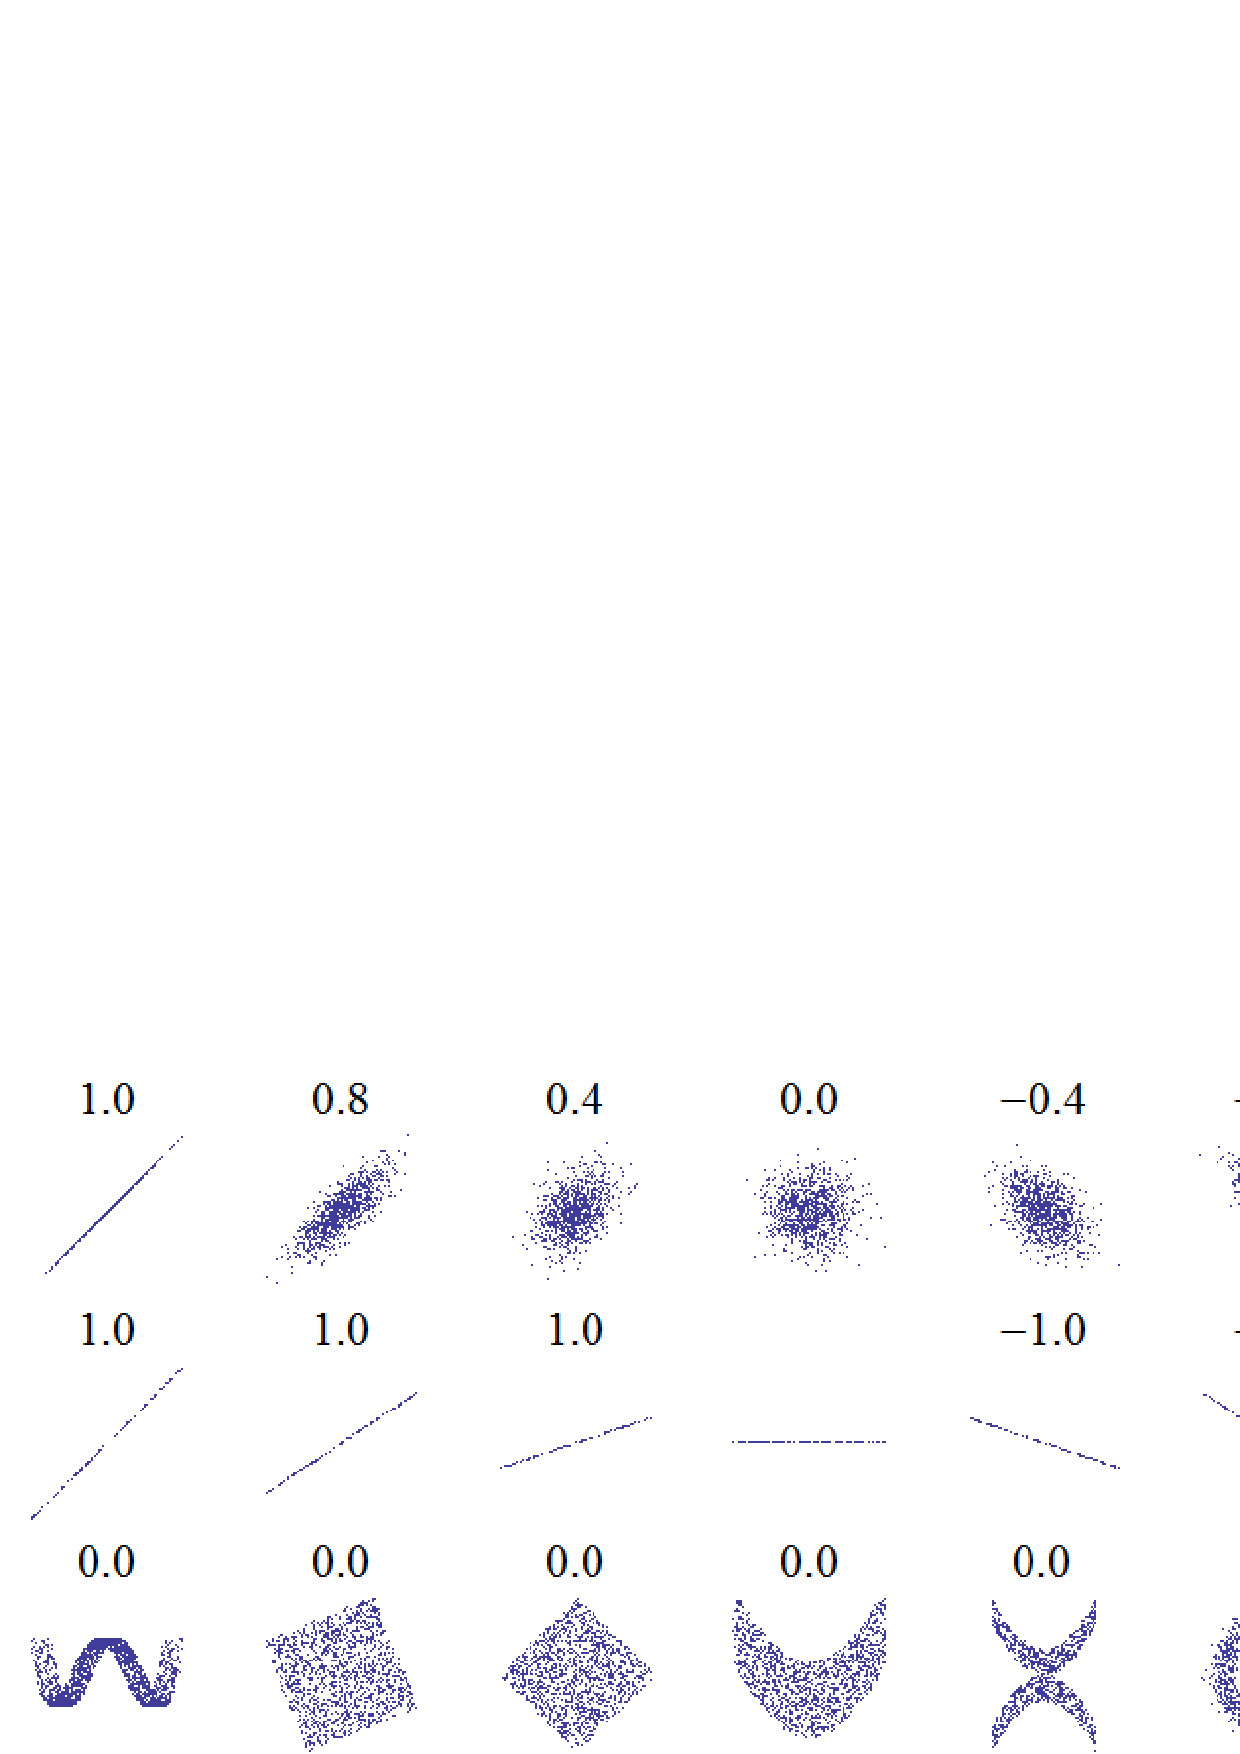
\includegraphics[height=2.5in]{figs/Correlation_examples.png}}
\caption{다양한 범위의 상관을 갖는 예제 데이터셋.}
\label{corr_examples}
\end{figure}

그림~\ref{corr_examples}은 \url{http://wikipedia.org/wiki/Correlation_and_dependence} 위키피디아 사이트에서 가져왔다.
그림에서 의도적으로 생성된 데이터셋에 대한 산점도와 상관 계수가 보여진다.
\index{산점도 (scatter plot)}
\index{그림 (plot)!산점 (scatter)}

상단 줄에는 다양한 상관계수를 가진 선형 관계를 보여준다; 상단 행에서 다양한 $\rho$ 값이 어떤 느낌인지 감을 얻을 수 있다.
두번째 행이 다양한 기울기를 가진 완전 상관의 예가 있다. 상관이 기울기와 관련이 없다는 것을 보여준다 (곧 기울기를 추정하는 것에 대해 언급할 것이다.) 세번째 행은 명확하게 관련이 있는 변수를 보여준다. 하지만, 관계가 비선형이라, 상관계수는 0이다.

\index{비선형 (nonlinear)}

상기 이야기의 교훈은 상관계수를 맹목적으로 계산하기 전에 데이터를 산점도를 그려서 항상 살펴봐야 한다는 것이다.

\index{상관 (correlation)}


\section{스피어만 순위 상관 (Spearman's rank correlation)}

피어슨 상관은 변수 사이의 관계가 선형이고, 변수가 대략 정규분포를 따른 다면 잘 동작한다. 하지만, 이상값이 존재하는 경우에는 강건하지 못하다.
스피어만 순위 상관이 대안으로 이상값과 기울어진 분포에 대한 효과를 완화한다. 
\index{피어슨 상관계수 (Pearson coefficient of correlation)}
\index{스피어만 상관계수 (Spearman coefficient of correlation)}
\index{정규분포 (normal distribution)}
\index{분포 (distribution)!정규 (normal)}
\index{가우스 분포 (Gaussian distribution)}
\index{분포 (distribution)!가우스 (Gaussian)}
\index{강건성 (robust)}
스피어만 상관을 계산하기 위해서 각 값의 {\bf 순위 (rank)}를 계산하는데 정렬된 표본에 인덱스에 해당한다.
예를 들어, 표본 {\tt [1, 2, 5, 7]}에서 값 5에 대한 순위는 3이다. 왜냐하면 정렬된 리스트에서 3번째 등장하기 때문이다. 그리고 나서 피어슨 순위 상관을 계산한다.

\index{왜도 (skewness)}
\index{이상값 (outlier)}
\index{순위 (rank)}

{\tt thinkstats2}는 스피어만 순위 상관을 계산하는 함수가 있다.

\begin{verbatim}
def SpearmanCorr(xs, ys):
    xranks = pandas.Series(xs).rank()
    yranks = pandas.Series(ys).rank()
    return Corr(xranks, yranks)
\end{verbatim}

인자를 판다스 시리즈 객체로 전환해서, 각 값에 대한 순위를 계산하고 시리즈를 반환하는 {\tt 순위 (rank)} 메쏘드를 사용할 수 있다. 
그리고 나서 {\tt Corr}을 사용해서 순위 상관을 계산한다.

\index{판다스 (pandas)}
\index{시리즈 (Series)}

직접적으로 {\tt Series.corr}을 사용해서 스피어만 메쏘드를 명세할 수도 있다.

\begin{verbatim}
def SpearmanCorr(xs, ys):
    xs = pandas.Series(xs)
    ys = pandas.Series(ys)
    return xs.corr(ys, method='spearman')
\end{verbatim}

BRFSS 데이터에 대한 스피어만 순위 상관계수는 0.54로 피어슨 상관계수 0.51보다 약간 더 높다. 차이에 대한 가능한 이유가 몇가지 있다:

\index{순위상관 (rank correlation)}
\index{BRFSS}

\begin{itemize}

\item 만약 관계가 비선형이면, 피어슨 상관은 관계의 강도를 과소추정하는 경향이 있다.
\index{비선형 (nonlinear)}

\item 만약 두 변수 분포중 하나가 기울거나(skewed) 이상점을 포함하게 되면, 피어슨 상관이 (어느 방향이든지) 영향을 받을 수 있다. 스피어만 상관계수가 좀더 강건하다.  

\index{기움 (skewness)}
\index{이상점 (outlier)}
\index{강건성 (robust)}

\end{itemize}

BRFSS 예제에서, 체중 분포가 대략 로그 정규분포라는 것을 알고 있다; 로그 변환을 통해서 정규 분포로 근사해서, 기울어짐이 없다.
기울어짐 효과를 제거하는 또다른 방법은 로그 취한 체중과 신장 사이 피어슨 상관을 계산하는 것이다.

\index{로그 정규분포 (lognormal distribution)}
\index{분포 (distribution)!로그 정규 (lognormal)}

\begin{verbatim}
    thinkstats2.Corr(df.htm3, np.log(df.wtkg2)))
\end{verbatim}

결과는 0.53으로 순위 상관계수 0.54에 가깝다. 그래서 이것이 의미하는 바는 체중 분포의 기울어짐이 피어슨과 스미어만 상관 사이 대부분 차이를 설명한다.
\index{기울어짐 (skewness)}
\index{스피어만 상관계수 (Spearman coefficient of correlation)}
\index{피어슨 상관계수 (Pearson coefficient of correlation)}


\section{상관과 인과 (Correlation and causation)}
\index{상관 (correlation)}
\index{인과 (causation)}

만약 변수 A와 B가 상관되었다면, 세가지 설명이 가능하다: A가 B의 발생 원인, B가 A의 발생 원인, 혹은 다른 요소가 A와 B의 발생 원인. 이와 같은 설명을 ``인과 관계 (causal relationships)''라고 부른다.
\index{인과 관계 (causal relationship)}

상관 그 자체로는 가능한 설명이 어느 것인지 구별하지는 못한다. 그래서, 어느 것이 사실인지 여러분에게 알려주지는 못한다. 이 원칙은 종종 다음 상용구로 표현된다. ``상관은 원인을 함축하지 않는다. (Correlation
does not imply causation)''.
애석하게도 자체 위키피디아 페이지도 있다. \url{http://wikipedia.org/wiki/Correlation_does_not_imply_causation}.

인과 증거를 제공하려면 무엇을 할 수 있을까요?

\begin{enumerate}

\item 시간을 사용한다. 만약 A가 B전에 온다면, A가 B를 발생시키는 원인 이지만, 다르게는 아니다. (적어도 인과에 관한 상식적인 이해에 따르면)
사건 순서는 인과 방향을 추론하는데 도움이 된다. 하지만, 다른 무언가 A와 B를 발생시키는 원인이 된다는 가능성을 배제하지 못한다.

\item 확률(randomness)을 사용한다. 만약 큰 표본을 임의로 두 집단으로 나누고 거의 모든 변수의 평균을 계산한다면, 차이는 작을 것으로 기대한다.
만약 한 변수를 제외하고 모든 변수에서 집단이 동일하다면, 허위 관계 (spurious relationship)을 제거할 수 있다.

\index{허위 관계 (spurious relationship)}

설사 관련 변수가 무엇인지 모른다고 하더라도 이 방식은 동작한다. 하지만, 관련 변수를 알고 있다면 더 잘 동작하는데 이유는 집단이 동일하다는 것을 확인할 수 있기 때문이다. 

\end{enumerate}

이와 같은 아이디어가 {\bf 무작위 대조군 시험 (randomized controlled
trial)}의 동기가 된다. 시험 대상이 임의로 두 (혹은 그 이상) 집단에 배속된다: {\bf 처리군 (treatment group)}은 신약 같은 일종의 개입을 받고, 
{\bf 대조군 (control group)}은 개입을 받지 않거나 효과가 알려진 또다른 처리를 받는다.

\index{무작위 대조군 시험 (randomized controlled trial)}
\index{대조군 시험 (controlled trial)}
\index{처리군 (treatment group)}
\index{대조군 (control group)}
\index{의학 (medicine)}

무작위 대조군 시험은 인과관계를 시연하는 가장 신뢰성 있는 방법이고, 과학-기반 의학의 초석이다. (\url{http://wikipedia.org/wiki/Randomized_controlled_trial} 참조).

불행하게도 대조군 시험은 실험실 과학, 의학, 그리고 몇몇 학문분야에서만 가능하다. 사회 과학에서, 대조군 실험이 드문데 이유는 불가능하거나 비윤리적이기 때문이다.
\index{윤리 (ethics)}

또 다른 대안은 {\bf 자연 실험 (natural experiment)}을 살펴보는 것인데, 다른 처리(treatment)가 유사한 집단에 적용된다. 자연 실험의 한가지 위험성은 명확하지 않는 방식으로 집단이 다를지도 모른다는 것이다.
이 주제에 대해서 웹사이트를 참조한다. \url{http://wikipedia.org/wiki/Natural_experiment}.
\index{자연 실험 (natural experiment)}

몇몇 경우에, {\bf 회귀 분석 (regression analysis)}을 사용해서 인과 관계를 추론할 수 있다. ~\ref{regression}장에서 다룰 것이다.
\index{회귀 분석 (regression analysis)}


\section{연습 문제}

이 연습문제 해답은 \verb"chap07soln.py"에 나와있다..

\begin{exercise}
NSFG 에서 나온 데이터를 사용해서,
출생체중과 산모연령 산점도를 그리시오.
출생체중과 산모연령 백분위수를 도식화하시오.
피어슨 상관과 스피어만 상관을 계산하시오.
두 번수 사이 관계를 어떻게 특징적으로 묘사할 수 있을까?
\index{출생체중}
\index{체중!출생}
\index{피어슨 상관계수}
\index{스피어만 상관계수}
\end{exercise}


\section{용어 사전}

\begin{itemize}

\item 산점도 (scatter plot): 두 변수 사이 관계를 데이터 각 행마다 점을 찍어 보임으로써 시각화.
\index{산점도 (scatter plot)}

\item 지터 (jitter): 시각화 목적으로 데이터에 추가되는 확률 잡음.
\index{지터 (jitter)}

\item 포화 (saturation): 다수의 점이 겹쳐지게 되어서 발생하는 정보 손실.
\index{포화 (saturation)}

\item 상관 (correlation): 두 변수 사이 관계 강도를 측정하는 통계량.
\index{상관 (correlation)}

\item 표준화(standardize): 변수 집합 값을 변환해서 평균 0, 분산 1로 만듦.
\index{표준화 (standardize)}

\item 표준 점수 (standard score): 표준화된 값으로, 평균에서 떨어진 표준편차로 표현.
\index{표준 점수 (standard score)}
\index{표준 편차 (standard deviation)}

\item 공분산 (covariance): 함께 변화하는 두 변수 경향성 측도.
\index{공분산 (covariance)}

\item 순위 (rank): 인덱스로, 정렬된 목록에 요소가 나타나는 순서.
\index{순위 (rank)}

\item 무작위 대조군 시험: 실험계획 (experimental design)으로 대상이 무작위 집단으로 나눠지고, 다른 집단에 다른 처리(treatment)가 주어진다.
\index{무작위 대조군 시험 (randomized controlled trial)}

\item 처리군 집단 (treatment group): 대조군 시험에서 일종의 개입(intervention)을 받는 집단.
\index{처리 집단 (treatment group)}

\item 대조군 집단 (control group): 대조군 시험에서 처리를 받지 않거나 이미 효과가 알려진 처리를 받는 집단.
\index{대조군 집단 (control group)}

\item 자연 실험 (natural experiment): 대상이 집단으로 자연 구분되는 현상을 이용하는 실험계획. 여기서 집단은 최소한 근사적으로 무작위가 된다.
\index{자연 실험 (natural experiment)}

\end{itemize}

